\begin{frame}{Voodoo: A Vector Algebra for Database Operations}
The overview of Voodoo
\begin{itemize}
\item A declarative intermediate algebra targeting in-memory databases
\item Abstracts hardware details
\item Vector oriented
\item Easy to generate low-level code (e.g. C/OpenCL)
\item Easy to be optimized (e.g. vectorization)
\end{itemize}
\end{frame}

\begin{frame}{Voodoo}
\begin{figure}[htb]
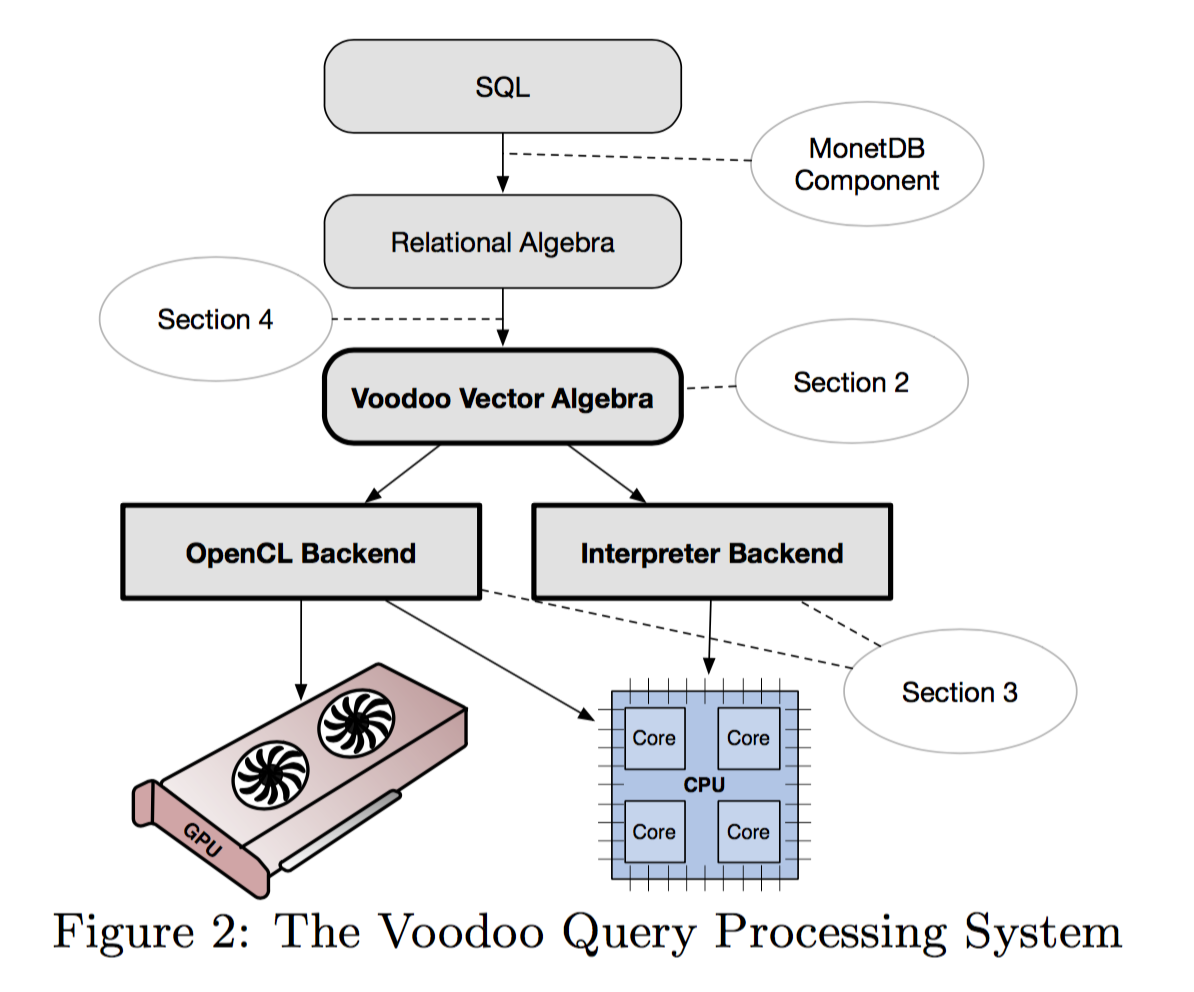
\includegraphics[width=0.85\textwidth]{fig/voodoo-fig2.png}
\end{figure}
\end{frame}

\begin{frame}[fragile]{Voodoo: Example}
Example 1: Multithreaded hierarchical aggregation in Voodoo

\begin{lstlisting}[basicstyle=\footnotesize]
1 input        := Load("input")
2 ids          := Range(input)
3 partitionSize:= Constant(1024)
4 positionIDs  := Divide(ids, partitionSize)
5 positions    := Partition(partitionIDs)
6 inputWPart   := Zip(input, partitionIDs)
7 partInput    := Scatter(inputWPart, positions)
8 pSum         := FoldSum(partInput.val,partInput.partition)
9 totalSum     := FoldSum(pSum)
\end{lstlisting}
\begin{itemize}
\item Line 3 and 4 create a vector that maps each tuple to a partition
\item Line 7 partitions the input according to positions
\item Line 8 and 9 performs aggregations on segments and the entire input respectively
\end{itemize}
\end{frame}

\begin{frame}[fragile]{Voodoo: Example}
Example 2: Adapt to SIMD in Voodoo, need to change
\begin{lstlisting}[basicstyle=\small]
line 3: laneCount    := Constant(2)
line 4: partitionIDs := Modulo(ids, laneCount)
\end{lstlisting}
\end{frame}

%\begin{itemize}
%\item Load: load a vector from persistent storage
%\item Range: generate a vector 1..step..n
%\item Zip: zip two vectors x,y into a new vector $\{(x_i, y_i)\}$
%\item Partition: generate a scatter position vector
%\end{itemize} 

\begin{frame}{Voodoo: Features}
Features
\begin{itemize}
\item Structured vectors (data): one-dimensional arrays
\item Controlled folding (a novel method): folding with a boolean mask
\item Operators in four categories: a rich set of operators
\end{itemize}
\end{frame}

\begin{frame}{Controlled folding}
\begin{figure}[htb]
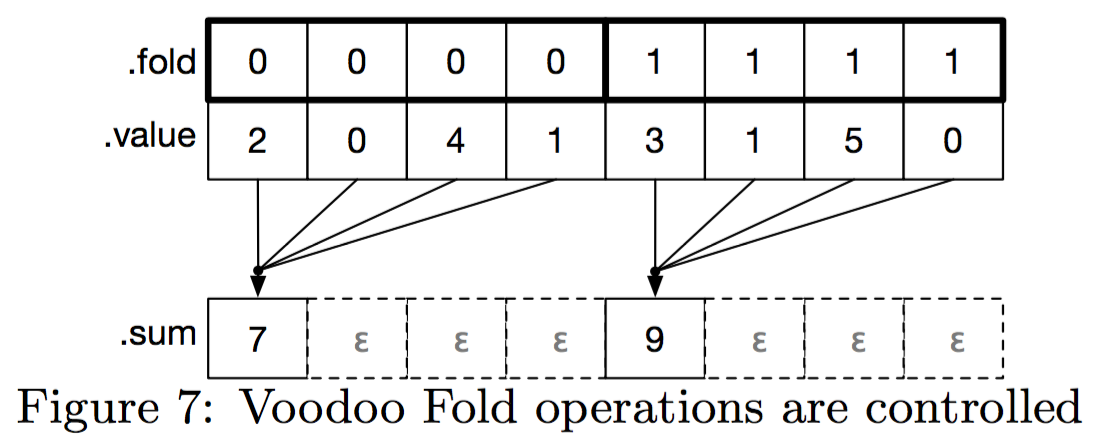
\includegraphics[width=0.7\textwidth]{fig/voodoo-fig7.png}
\end{figure}
\end{frame}

\begin{frame}[fragile]{Controlled folding}
The equivalent code in HorseIR is
\begin{lstlisting}[language=HorseIR, basicstyle=\footnotesize]
t0 = @compress(fold, value)
t1 = @sum(t0)
\end{lstlisting}
When generating code from HorseIR, the idea of controlled folding can be
applied by fusing this adjacent two lines of code.
\end{frame}

\begin{frame}{Voodoo Operators}
\begin{enumerate}
\item Maintenance operations: I/O, such as Load
\item Data-parallel operations: such as logical expressions
\item Fold operations: database specials
\item Shape operations: such as Range
\end{enumerate}

As far as we can see, the design of Voodoo intends to become database-friendly.
\end{frame}

\begin{frame}{OpenCL Back-end}
\begin{figure}[htb]
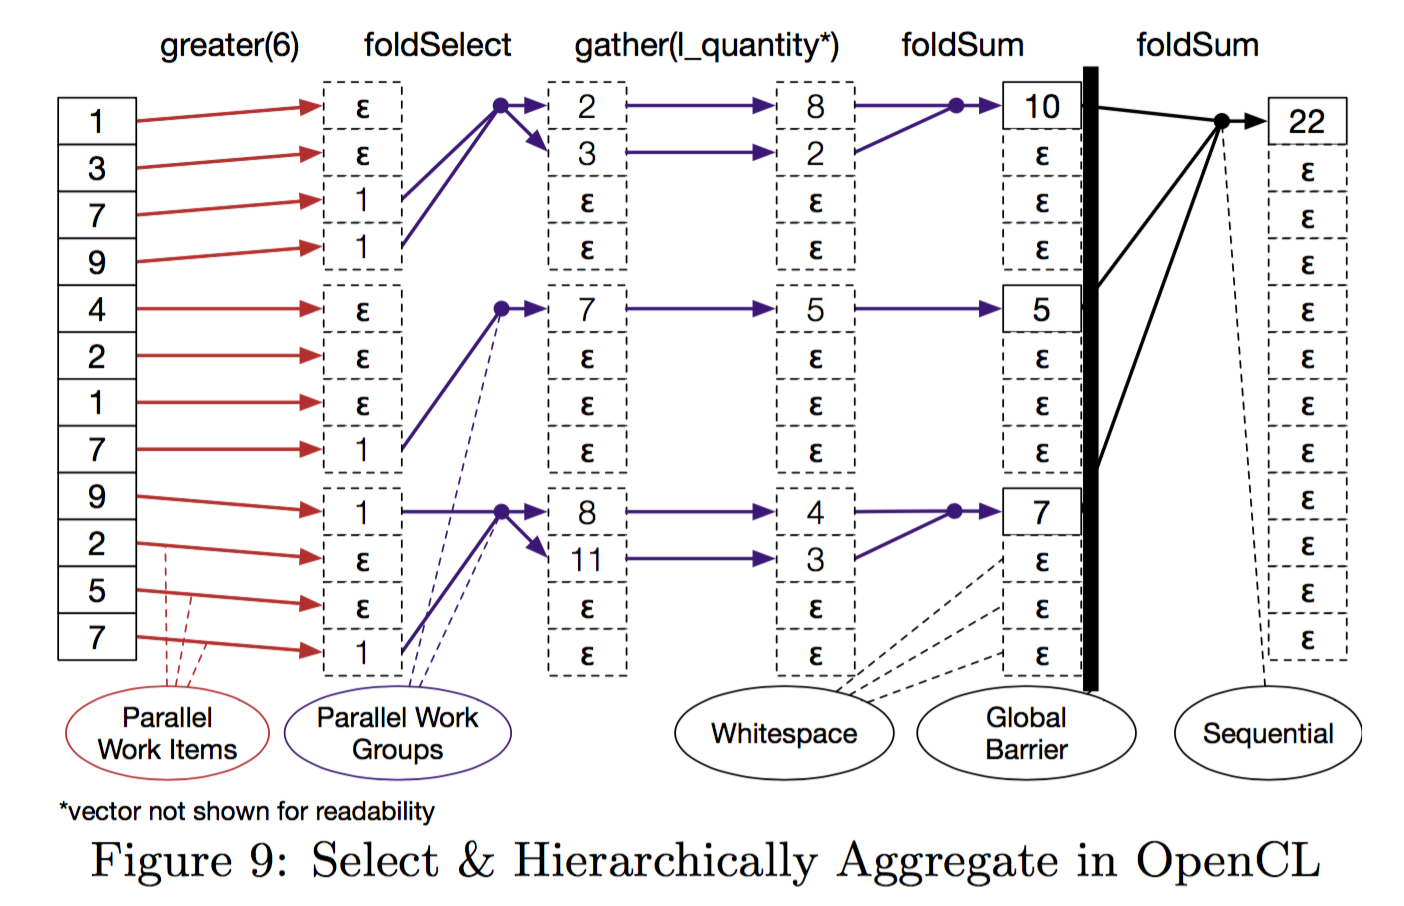
\includegraphics[width=0.8\textwidth]{fig/voodoo-fig9.png}
\end{figure}
\end{frame}

\begin{frame}{Evaluation}
Setup
\begin{itemize}
\item TPC-H benchmarks
\item GPU: MonetDB/Ocelot vs. Voodoo/GPU
\item CPU: HyPeR vs. Voodoo/CPU
\item Only the execution time counted
\end{itemize}
\end{frame}

\begin{frame}{Evaluation: GPU}
\begin{figure}[htb]
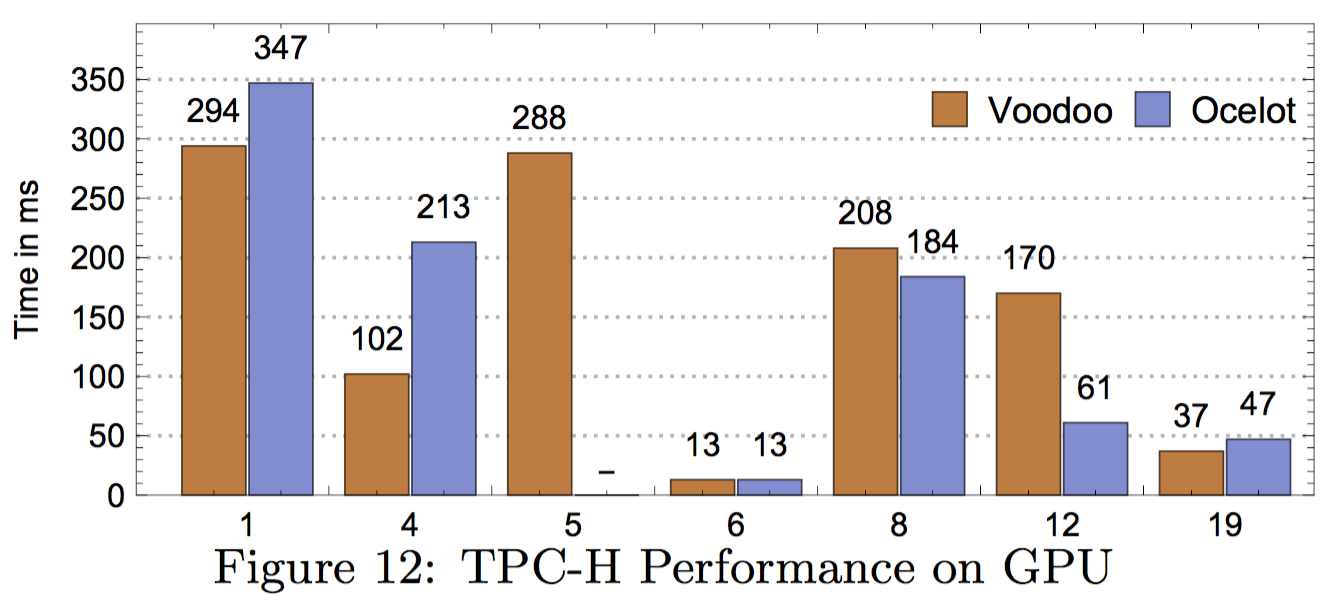
\includegraphics[width=0.8\textwidth]{fig/voodoo-fig12.png}
\end{figure}
\begin{itemize}
\item Voodoo \textgreater\ Ocelot in 3 queries (q1/4/19)
\end{itemize} 
\end{frame}

\begin{frame}{Evaluation: CPU}
\begin{figure}[htb]
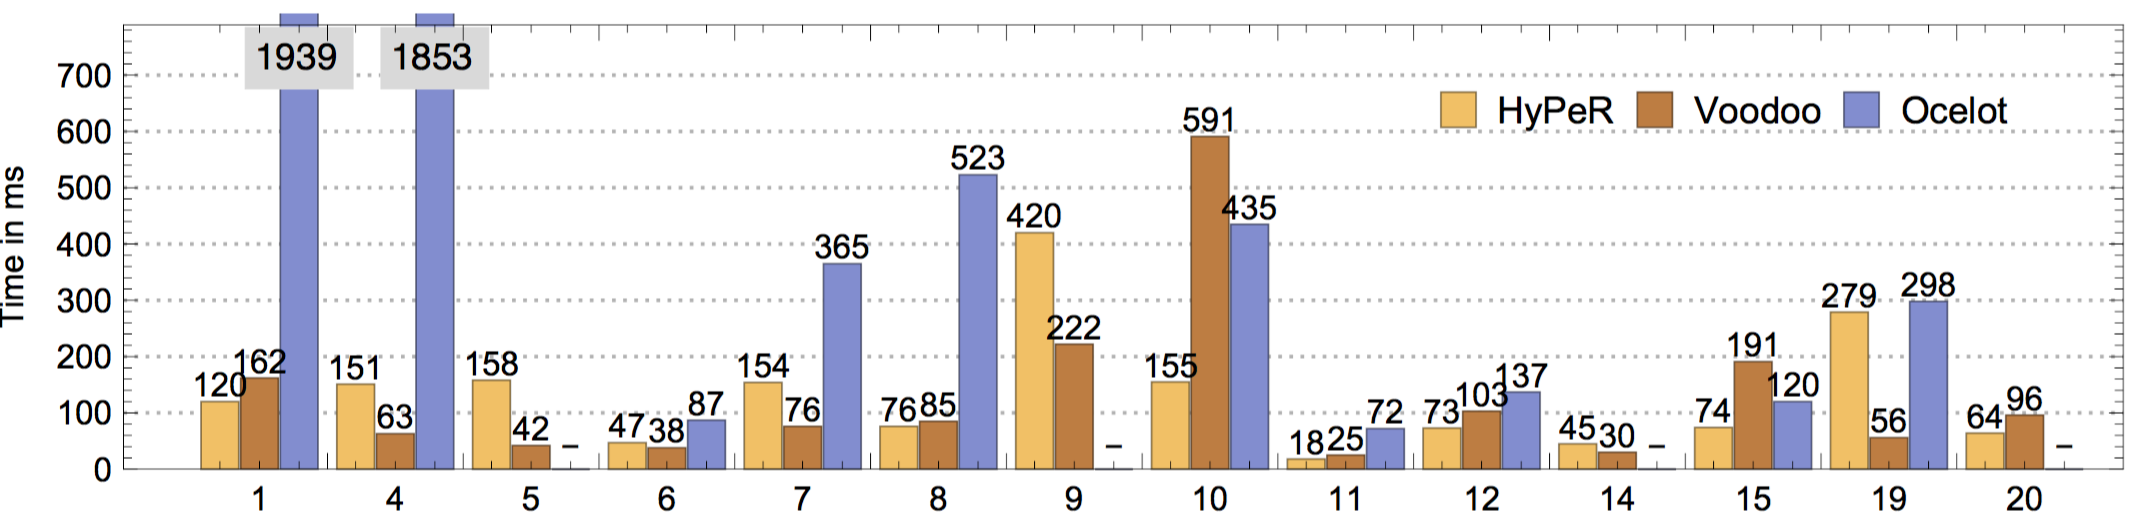
\includegraphics[width=1\textwidth]{fig/voodoo-fig13.png}
\end{figure}
\begin{itemize}
\item HyPeR and Ocelot target CPU and GPU respectively
\item Observation: HyPeR \textgreater Voodoo (7), HyPeR \textless Voodoo (7)
\end{itemize} 
\end{frame}

\begin{frame}{Summary}
Brief summary
\begin{itemize}
\item Voodoo is an intermediate vector algebra
\item The paper presents a novel technique: control vectors
\item Voodoo makes it easy to explore optimizations for different architectures
\end{itemize} 
\pause
However, we can see some restrictions:
\begin{itemize}
\item No support for non-homogeneous data, such as lists
\item No systemic design of operators (build-in functions)
\item Thus, not easy for optimizations on the level of Voodoo
\end{itemize} 
\end{frame}

